\section{DTP-Dijagram toka podataka}

Dijagrami toka podataka opisuju kretanje podataka kroz sistem. Predstavlja tok podataka kroz procese u kojima učestvuju entiteti. Dijagrami toka podataka se mogu raditi na više nivoa. DTP nivoa 0 opisuje ceo sistem kao jednu celinu. Niži nivoi predstavljaju specijalizaciju nivoa viših nivoa.Tok podataka kroz sistem se
predstavlja strelicama. Neki od podataka, nastalih u procesu, se čuvaju u bazi podataka.

\begin{figure}[ht]
\centering
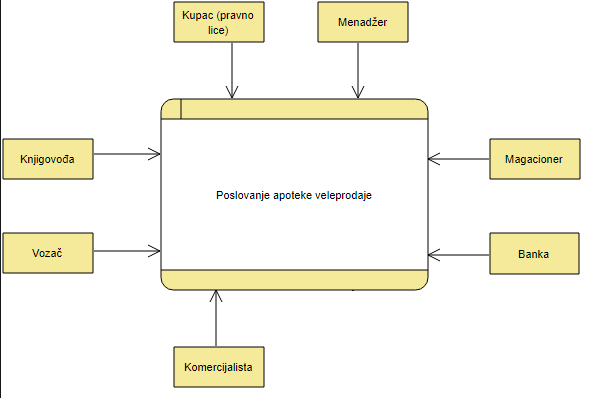
\includegraphics{slike/dtp-lvl0.png}%
\caption{DTP nivoa 0}
\end{figure}

\begin{figure}[ht]
\centering
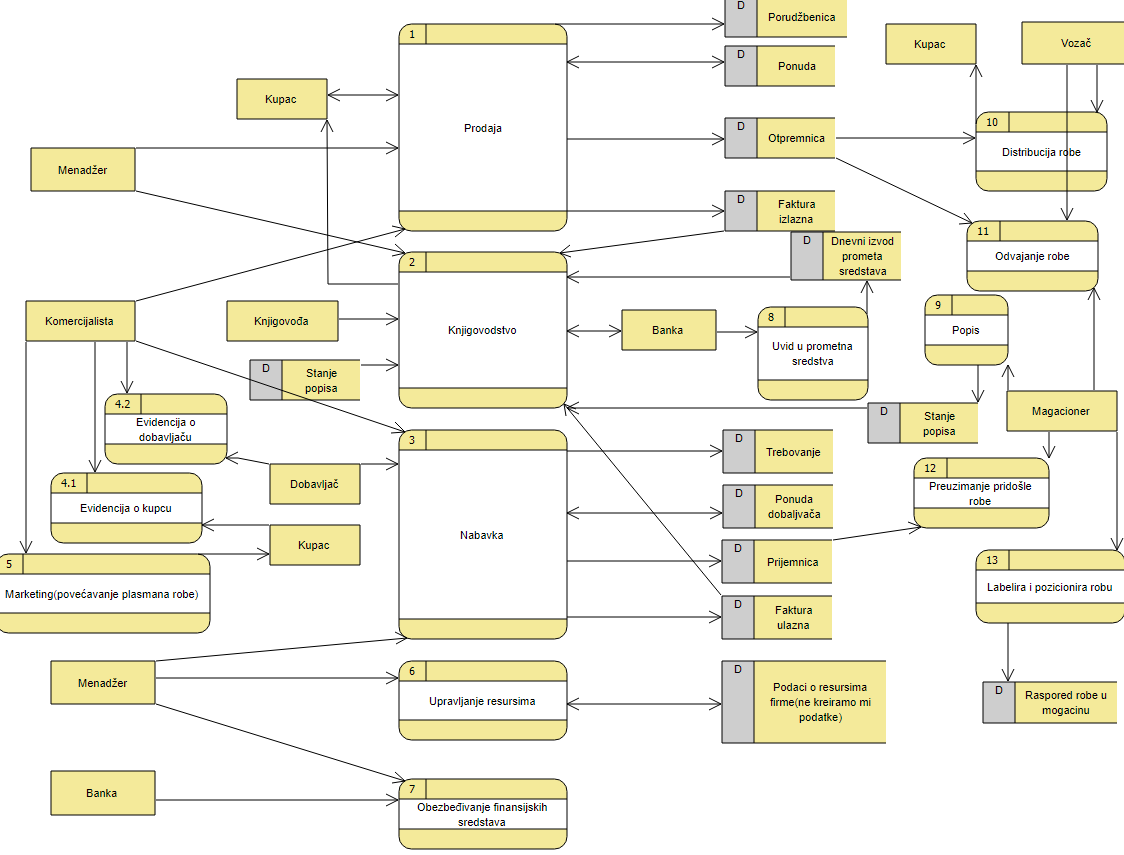
\includegraphics[width=170mm]{slike/dtp-lvl1.png}%
\caption{DTP nivoa 1}
\end{figure}


\begin{figure}[ht]
\centering
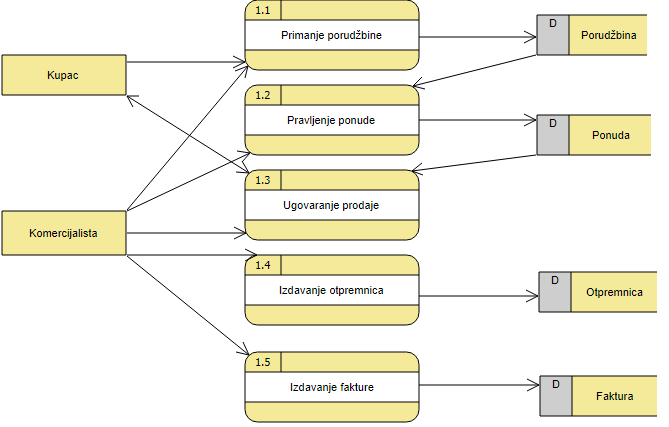
\includegraphics[width=170mm]{slike/dtp-lvl2prodaja.png}%
\caption{DTP nivoa 2}
\end{figure}

\begin{figure}[ht]
\centering
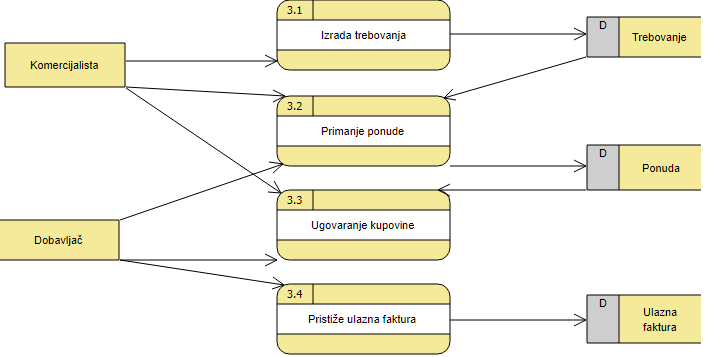
\includegraphics[width=170mm]{slike/dtp-lvl2nabavka.png}%
\caption{DTP nivoa 2}
\end{figure}

\begin{figure}[ht]
\centering
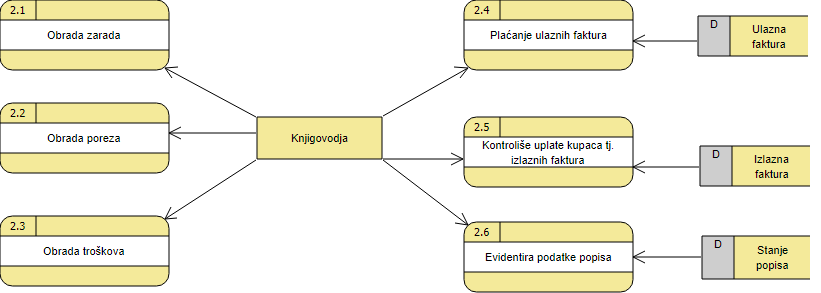
\includegraphics[width=170mm]{slike/dtp-lvl2knjig.png}%
\caption{DTP nivoa 2}
\end{figure}

\clearpage